\chapter{\subspacesTitle}\label{subspacesspanning}

It is time to study vector spaces more carefully and return to  some fundamental questions:

\begin{enumerate}
\item \emph{Subspaces}: When is a subset of a vector space itself a vector space?  (This is the notion of a \emph{subspace}.)

\item \emph{Linear Independence}: Given a collection of vectors, is there a way to tell whether they are independent, or if one is a ``linear combination'' of the others? 

\item \emph{Dimension}: Is there a consistent definition of how ``big'' a vector space is?

\item \emph{Basis}:  How do we label vectors?  Can we write any vector as a sum of some basic set of vectors?  How do we change our point of view from vectors labeled one way to vectors labeled in another way?
\end{enumerate}
\index{Subspace!notion of}\index{Linear independence!concept of}\index{Dimension!notion of}\index{Basis!concept of}
Let's start at the top!

\section{Subspaces}

\begin{definition}
We say that a subset $U$ of a vector space $V$ is a {\bf subspace}\index{Subspace} of $V$ if $U$ is a vector space under the inherited addition and scalar multiplication operations of $V$. 
\end{definition}

\begin{example}
Consider a plane $P$ in $\Re^3$ through the origin:
\[
ax+by+cz=0.
\]

\begin{center}
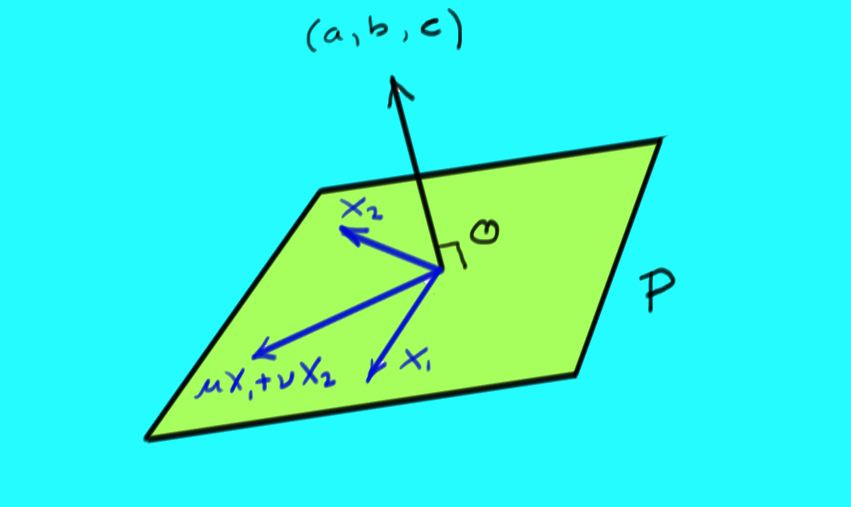
\includegraphics[scale=.3]{\subspacesPath/subspace_plane.jpg}
\end{center}
This equation can be expressed as the homogeneous system $\rowvec{a & b & c}\colvec{x\\y\\z}=0$, or $MX=0$ with $M$ the matrix $\rowvec{a & b & c}$.  If $X_1$ and $X_2$ are both solutions to $MX=0$, then, by linearity of matrix multiplication, so is $\mu X_1 + \nu X_2$:
\[
M(\mu X_1 + \nu X_2) = \mu MX_1 + \nu MX_2 = 0.
\]
So $P$ is closed under addition and scalar multiplication.  Additionally, $P$ contains the origin (which can be derived from the above by setting $\mu=\nu=0$).  All other vector space requirements hold for $P$ because they hold for all vectors in $\Re^3$.
\end{example}


%\begin{figure}
%\begin{center}
%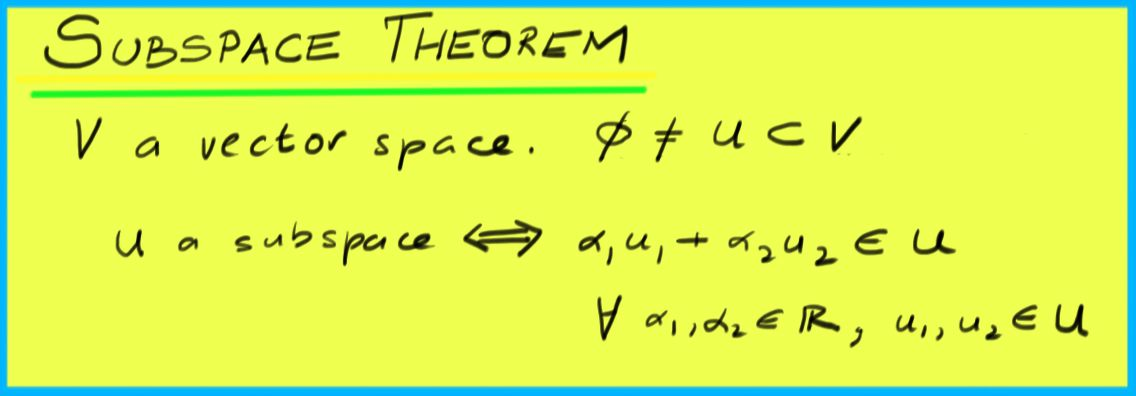
\includegraphics[scale=.33]{\subspacesPath/subspace_thm.jpg}
%\end{center}
%\end{figure}

\begin{theorem}[\hypertarget{sst}{Subspace Theorem}]\index{Subspace theorem}\label{subspacetheorem}
Let $U$ be a non-empty subset of a vector space $V$.  Then $U$ is a subspace if and only if $\mu u_1 + \nu u_2 \in U$ for arbitrary $u_1, u_2$ in $U$, and arbitrary constants $\mu, \nu$.  
\end{theorem}

\begin{proof}
One direction of this proof is easy: if \(U\) is a subspace, then it is a vector space, and so by the additive closure and multiplicative closure properties of vector spaces, it has to be true that \(\mu u_1 + \nu u_2 \in U\) for all \(u_1,u_2\) in \(U\) and all constants constants \(\mu, \nu\).

The other direction is almost as easy: we need to show that if \(\mu u_1 + \nu u_2 \in U\) for all \(u_1, u_2\) in \(U\) and all constants \(\mu, \nu\), then \(U\) is a vector space. That is, we need to show that the \hyperref[vectorspace]{ten properties of vector spaces} are satisfied. We already know that the additive closure and multiplicative closure properties are satisfied. Further, \(U\) has all of the other eight properties  because \(V\) has them. \end{proof}

\noindent
Note that the requirements of the subspace theorem are often referred to as ``closure''\index{Closure}.

%From now on, w
We can use this theorem to check if a set is a vector space. That is, if we have some set \(U\) of vectors that come from some bigger vector space \(V\), to check if \(U\) itself forms a smaller vector space we need check only two things: 
\begin{enumerate}
\item If we add any two vectors in \(U\), do we end up with a vector in \(U\)?
\item If we multiply any vector in \(U\) by any constant, do we end up with a vector in \(U\)? 
\end{enumerate}
If the answer to both of these questions is yes, then \(U\) is a vector space. If not, \(U\) is not a vector space.

%\begin{center}\href{\webworkurl ReadingHomework15/1/}{Reading homework: problem \ref{subspacesspanning}.1}\end{center}
\Reading{SubspacesAndSpans}{1}


\section{Building Subspaces}

Consider the set 
\[
U= \left\{ \colvec{1\\0\\0}, \colvec{0\\1\\0} \right\} \subset \Re^3.
\]
Because $U$ consists of only two vectors, it clear that $U$ is \emph{not} a vector space, since any constant multiple of these vectors should also be in $U$.  For example, the $0$-vector is not in $U$, nor is $U$ closed under vector addition.

But we know that any two vectors define a plane:
\begin{center}
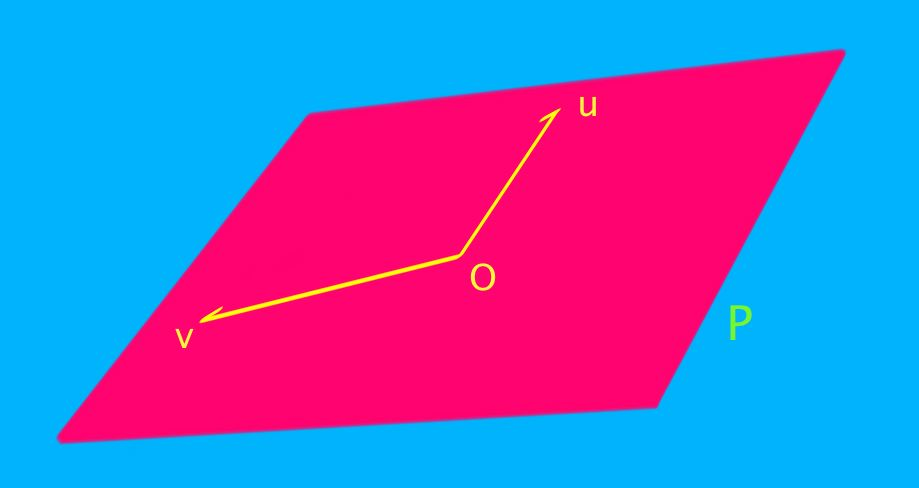
\includegraphics[scale=.3]{\subspacesPath/span_plane.jpg}
\end{center}
 In this case, the vectors in $U$ define the $xy$-plane in $\Re^3$.  We can view the $xy$-plane as the set of all vectors that arise as a linear combination of the two vectors in $U$.  We call this set of all linear combinations the \emph{span}\index{Span} of $U$:
\[
\spa(U)=\left\{ x \colvec{1\\0\\0}+y \colvec{0\\1\\0} \middle| x,y\in \Re \right\}.
\]
Notice that any vector in the $xy$-plane is of the form
\[
\colvec{x\\y\\0} = x \colvec{1\\0\\0}+y \colvec{0\\1\\0} \in \spa(U).
\]

\begin{definition}
Let $V$ be a vector space and $S=\{ s_1, s_2, \ldots \} \subset V$ a subset of~$V$.  Then the {\bf span of $S$}, denoted $\spa(S)$, is the set
\[
\spa(S):=\{ r^1s_1+r^2s_2+\cdots + r^Ns_N ~|~ r^i\in \Re, N\in \N \}.
\]
\end{definition}

That is, the span of \(S\) is the set of all finite linear combinations\footnote{Usually our vector spaces are defined over \(\mathbb{R}\), but in general we can have vector spaces defined over different base fields such as \(\mathbb{C}\) or \(\mathbb{Z}_2\). The coefficients \(r^i\) should come from whatever our base field is (usually \(\mathbb{R}\)).} of elements of \(S\). Any {\it finite} sum of the form ``a constant times \(s_1\) plus a constant times \(s_2\) plus a constant times \(s_3\) and so on'' is in the span of \(S\).\footnote{It is important that we only allow finitely many terms in our linear combinations; in the definition above, \(N\) must be a finite number. It can be any finite number, but it must be finite. We can relax the requirement that $S=\{s_1,s_2,\ldots\}$ and just let $S$ be any set of vectors. Then we shall write $\spa(S):=\{ r^1s_1+r^2s_2+\cdots + r^Ns_N ~|~ r^i\in \Re, s_i\in S, N\in \N, \}$
 }.

\begin{example}
Let $V=\Re^3$ and $X\subset V$ be the $x$-axis.  Let $P=\colvec{0\\1\\0}$, and set $$S=X \cup \{P\}\, .$$
The vector \(\colvec{2 \\ 3 \\ 0}\) is in \(\spa(S),\) because \(\colvec{2\\3\\0}=\colvec{2\\0\\0}+3\colvec{0\\1\\0}.\) Similarly, the vector \(\colvec{-12 \\ 17.5 \\ 0}\) is in \(\spa(S),\) because \(\colvec{-12\\17.5\\0}=\colvec{-12\\0\\0}+17.5\colvec{0\\1\\0}.\)
Similarly, any vector of the form
\[
\colvec{x\\0\\0}+y \colvec{0\\1\\0} = \colvec{x\\y\\0}
\]
is in \(\spa(S)\). On the other hand, any vector in \(\spa(S)\) must have a zero in the \(z\)-coordinate. (Why?) 
So $\spa(S)$ is the $xy$-plane, which is a vector space.  (Try drawing a picture to verify this!)
\end{example}

%\begin{center}\href{\webworkurl ReadingHomework15/2/}{Reading homework: problem \ref{subspacesspanning}.2}\end{center}
\Reading{SubspacesAndSpans}{2}

\begin{lemma}
For any subset $S\subset V$, $\spa(S)$ is a subspace of $V$.
\end{lemma}

\begin{proof}
We need to show that $\spa(S)$ is a vector space.

It suffices to show that $\spa(S)$ is closed under linear combinations.  Let $u,v\in \spa(S)$ and $\lambda, \mu$ be constants.  By the definition of $\spa(S)$, there are constants $c^i$ and $d^i$ (some of which could be zero) such that:
\begin{eqnarray*}
u & = & c^1s_1+c^2s_2+\cdots \\
v & = & d^1s_1+d^2s_2+\cdots \\
\Rightarrow \lambda u + \mu v & = & \lambda (c^1s_1+c^2s_2+\cdots ) + \mu (d^1s_1+d^2s_2+\cdots ) \\
& = & (\lambda c^1+\mu d^1)s_1 + (\lambda c^2+\mu d^2)s_2 + \cdots
\end{eqnarray*}
This last sum is a linear combination of elements of $S$, and is thus in $\spa(S)$.  Then $\spa(S)$ is closed under linear combinations, and is thus a subspace of~$V$.
\end{proof}

Note that this proof, like many proofs, consisted of little more than just writing out the definitions.



\begin{example}
For which values of $a$ does

\[
\spa \left\{ \colvec{1\\0\\a} , \colvec{1\\2\\-3} , \colvec{a\\1\\0}   \right\} = \Re^3?
\]
Given an arbitrary vector $\colvec{x\\y\\z}$ in $\Re^3$, we need to find constants $r^1, r^2, r^3$ such that 

\[
r^1 \colvec{1\\0\\a} + r^2\colvec{1\\2\\-3} +r^3 \colvec{a\\1\\0} = \colvec{x\\y\\z}.
\]
We can write this as a linear system in the unknowns $r^1, r^2, r^3$ as follows:

\[
\begin{pmatrix}
1 & 1 & a \\ 
0 & 2 & 1 \\
a & -3 & 0
\end{pmatrix}
\colvec{r^1\\r^2\\r^3}
= \colvec{x\\y\\z}.
\]
If the matrix $M=\begin{pmatrix}
1 & 1 & a \\ 
0 & 2 & 1 \\
a & -3 & 0
\end{pmatrix}$ is invertible, then we can find a solution 
\[
M^{-1}\colvec{x\\y\\z}=\colvec{r^1\\r^2\\r^3}
\]
for \emph{any} vector $\colvec{x\\y\\z} \in \Re^3$.

Therefore we should choose $a$ so that $M$ is invertible:  

\[
i.e.,\;  0 \neq \det M = -2a^2 + 3 + a = -(2a-3)(a+1). 
\]
Then the span is $\Re^3$ if and only if $a \neq -1, \frac{3}{2}$.
\end{example}

\Videoscriptlink{subspaces_and_spanning_sets_example.mp4}{Linear systems as spanning sets}{scripts_subspaces_and_spanning_sets_example}

Some other very important ways of building subspaces are given in the following examples.

\begin{example}
(The kernel of a linear map).\\[-2mm]

\noindent
Suppose $L:U\to V$ is a linear map between vector spaces. Then if
$$
L(u)=0=L(u')\, ,
$$
linearity tells us that
$$
L(\alpha u + \beta u') = \alpha L(u) + \beta L(u') =\alpha 0 + \beta 0 = 0\, .
$$
Hence, thanks to the subspace theorem,  the set of all vectors in $U$ that are mapped to the zero vector is a subspace of $V$.
It is called the kernel of $L$:
$$
{\rm ker} L:=\{u\in U| L(u) = 0\}\subset U.
$$
Note that finding a kernel means finding a solution to a homogeneous linear equation. 
\end{example}

\begin{example}
(The image of a linear map).\\[-2mm]

\noindent
Suppose $L:U\to V$ is a linear map between vector spaces. Then if
$$
v=L(u) \mbox{ and } v'=L(u')\, ,
$$
linearity tells us that
$$
\alpha v + \beta v' = \alpha L(u) + \beta L(u') =L(\alpha u +\beta u')\, .
$$
Hence, calling once again on the subspace theorem,  the set of all vectors in $V$ that are obtained as outputs of the
map $L$ is a subspace.
It is called the image of $L$:
$$
{\rm im} L:=\{L(u) \ |\  u\in U \}\subset V.
$$
\end{example}

\begin{example}
(An eigenspace of a linear map).\\[-2mm]

\noindent
Suppose $L:V\to V$ is a linear map and $V$ is a vector space. Then if
$$
L(u)=\lambda u \mbox{ and } L(v)=\lambda v\, ,
$$
linearity tells us that
$$
L(\alpha u + \beta v) = \alpha L(u) + \beta L(v) =\alpha L(u) + \beta L(v) =\alpha \lambda u  + \beta \lambda v = \lambda (\alpha u + \beta v)\, .
$$
Hence, again by subspace theorem, the set of all vectors in $V$ that
obey the {\it eigenvector equation} $L(v)=\lambda v$ is a subspace of $V$. 
It is called an eigenspace
$$
V_\lambda:=\{v\in V| L(v) = \lambda v\}.
$$
For most scalars $\lambda$, the only solution to $L(v) = \lambda v$ will be $v=0$, which yields the trivial subspace $\{0\}$.
When there are nontrivial solutions to $L(v)=\lambda v$, the number~$\lambda$ is called an eigenvalue, and carries
essential information about the map~$L$. 
\end{example}

Kernels, images and eigenspaces are discussed in great depth in chapters~\ref{kernelrank} and~\ref{eigenvalseigenvects}.


%\section*{References}
%Hefferon, Chapter Two, Section I.2: Subspaces and Spanning Sets
%\\
%Beezer, Chapter VS, Section S
%\\
%Beezer, Chapter V, Section LC
%\\
%Beezer, Chapter V, Section SS
%\\
%Wikipedia:
%\begin{itemize}
%\item \href{http://en.wikipedia.org/wiki/Linear_subspace}{Linear Subspace}
%\item \href{http://en.wikipedia.org/wiki/Linear_span}{Linear Span}
%\end{itemize}
%

\section{Review Problems}
{\bf Webwork:} 
\begin{tabular}{|c|c|}
\hline
Reading Problems & 
 \hwrref{SubspacesAndSpans}{1}, \hwrref{SubspacesAndSpans}{2}\\
 Subspaces &\hwref{SubspacesAndSpans}{3},
 \hwref{SubspacesAndSpans}{4},
 \hwref{SubspacesAndSpans}{5},
 \hwref{SubspacesAndSpans}{6}\\
 Spans &\hwref{SubspacesAndSpans}{7},
 \hwref{SubspacesAndSpans}{8}\\
  \hline
\end{tabular}







\begin{enumerate}
\item \label{det33} Let $M=\begin{pmatrix}
m^1_1 & m^1_2 & m^1_3\\
m^2_1 & m^2_2 & m^2_3\\
m^3_1 & m^3_2 & m^3_3\\
\end{pmatrix}$.  Use row operations to put $M$ into \emph{row echelon form}.  For simplicity, assume that $m_1^1\neq 0 \neq m^1_1m^2_2-m^2_1m^1_2$.

Prove that $M$ is non-singular if and only if:
\[
m^1_1m^2_2m^3_3 
- m^1_1m^2_3m^3_2 
+ m^1_2m^2_3m^3_1 
- m^1_2m^2_1m^3_3 
+ m^1_3m^2_1m^3_2
- m^1_3m^2_2m^3_1
\neq 0
\]

\phantomnewpage

\item 
\begin{enumerate}
\item What does the matrix $E^1_2=\begin{pmatrix}
0 & 1 \\
1 & 0
\end{pmatrix}$ do to $M=\begin{pmatrix}
a & b \\
d & c
\end{pmatrix}$ under left multiplication?  What about right multiplication?
\item Find elementary matrices $R^1(\lambda)$ and $R^2(\lambda)$ that respectively multiply rows $1$ and $2$ of $M$ by $\lambda$ but otherwise leave $M$ the same under left multiplication.
\item Find a matrix $S^1_2(\lambda)$ that adds a multiple $\lambda$ of row $2$ to row $1$ under left multiplication.
\end{enumerate}

\phantomnewpage

\item Let $M$ be a matrix and $S^i_jM$ the same matrix with rows \(i\) and \(j\) switched.  Explain every line of the 
\hyperlink{rowswap}{series of equations} proving that $\det M = -\det (S^i_jM)$.

\phantomnewpage

%\item \label{prob_inversion_number} This problem is a ``hands-on'' look at why \hyperlink{permutation_parity}{the property} describing the parity of permutations is true.
%
%\hypertarget{inversion_number}{The \emph{inversion number}}\index{Permutation!Inversion number} of a permutation $\sigma$ is the number of pairs $i<j$ such that $\sigma(i)>\sigma(j)$; it's the number of ``numbers that appear left of smaller numbers'' in the permutation.  For example, for the permutation $\rho = [4,2,3,1]$, the inversion number is $5$. The number $4$ comes before $2,3,$ and $1$, and $2$ and $3$ both come before $1$.
%
%Given a permutation $\sigma$, we can make a new permutation $\tau_{i,j} \sigma$ by exchanging the $i$th and $j$th entries of $\sigma$.
%
%\begin{enumerate}
%\item What is the inversion number of the permutation \(\mu=[1,2,4,3]\) that exchanges 4 and 3 and leaves everything else alone? Is it an even or an odd permutation?
%
%\item What is the inversion number of the permutation \(\rho=[4,2,3,1]\) that exchanges 1 and 4 and leaves everything else alone? Is it an even or an odd permutation?
%
%\item What is the inversion number of the permutation \(\tau_{1,3} \mu\)? Compare the parity\footnote{The \emph{parity} of an integer refers to whether the integer is even or odd. Here the parity of a permutation $\mu$ refers to the parity of its inversion number.} of \(\mu\) to the parity of \(\tau_{1,3} \mu.\)
%
%\item What is the inversion number of the permutation \(\tau_{2,4} \rho\)? Compare the parity of \(\rho\) to the parity of \(\tau_{2,4} \rho.\)
%
%\item What is the inversion number of the permutation \(\tau_{3,4} \rho\)? Compare the parity of \(\rho\) to the parity of \(\tau_{3,4} \rho.\)
%\end{enumerate}
%
%\videoscriptlink{elementary_matrices_determinant_hint.mp4}{Problem~\ref{prob_inversion_number} hints}{scripts_elementary_matrices_determinants_hint}

\phantomnewpage

%\item \label{problem_permutation} (Extra credit) Here we will examine a (very) small set of the general properties about permutations and their applications. In particular, we will show that one way to compute the sign of a permutation is by finding the \hyperlink{inversion_number}{inversion number} $N$ of $\sigma$ and we have
%\[
%\sgn(\sigma) = (-1)^N.
%\]
%
%For this problem, let $\mu = [1,2,4,3]$.
%
%\begin{enumerate}
%\item Show that every permutation $\sigma$ can be sorted by only taking simple (adjacent) transpositions\index{Permutation!Simple transposition} $s_i$ where $s_i$ interchanges the numbers in position $i$ and $i+1$ of a permutation $\sigma$ (in our other notation $s_i = \tau_{i,i+1}$). For example $s_2 \mu = [1, 4, 2, 3]$, and to sort $\mu$ we have $s_3 \mu = [1, 2, 3, 4]$.
%
%\item \label{prob_part_relations} We can compose simple transpositions together to represent a permutation (note that the sequence of compositions is not unique), and these are associative, we have an identity (the trivial permutation where the list is in order or we do nothing on our list), and we have an inverse since it is clear that $s_i s_i \sigma = \sigma$. Thus permutations of $[n]$ under composition are an example of a \hyperref[groups]{group}. However note that not all simple transpositions commute with each other since
%\begin{align*}
%s_1 s_2 [1, 2, 3] & = s_1 [1, 3, 2] = [3, 1, 2]
%\\ s_2 s_1 [1, 2, 3] & = s_2 [2, 1, 3] = [2, 3, 1]
%\end{align*}
%(you will prove here when simple transpositions commute). When we consider our initial permutation to be the trivial permutation $e = [1, 2, \dotsc, n]$, we do not write it; for example $s_i \equiv s_i e$ and $\mu = s_3 \equiv s_3 e$. This is analogous to not writing 1 when multiplying. Show that $s_i s_i = e$ (in shorthand $s_i^2 = e$), $s_{i+1} s_i s_{i+1} = s_i s_{i+1} s_i$ for all $i$, and $s_i$ and $s_j$ commute for all $|i - j| \geq 2$.
%
%\item Show that every way of expressing $\sigma$ can be obtained from using the relations proved in part~\ref{prob_part_relations}. In other words, show that for any expression $w$ of simple transpositions representing the trivial permutation $e$, using the proved relations.
%
%\emph{Hint: Use induction on $n$. For the induction step, follow the path of the $(n+1)$-th strand by looking at $s_n s_{n-1} \cdots s_k s_{k\pm1} \cdots s_n$ and argue why you can write this as a subexpression for any expression of $e$. Consider using diagrams of these paths to help.}
%
%\item The simple transpositions \hyperlink{action}{acts on} an $n$-dimensional vector space $V$ by $s_i v = E^i_{i+1} v$ (where $E^i_j$ is \hyperlink{elem_matrix_row_swap}{an elementary matrix}) for all vectors $v \in V$. Therefore we can just represent a permutation $\sigma$ as the matrix $M_{\sigma}$\footnote{Often people will just use $\sigma$ for the matrix when the context is clear.}, and we have $\det(M_{s_i}) = \det(E^i_{i+1}) = -1$. Thus prove that $\det(M_{\sigma}) = (-1)^N$ where $N$ is a number of simple transpositions needed to represent $\sigma$ as a permutation. You can assume that $M_{s_i s_j} = M_{s_i} M_{s_j}$ (it is not hard to prove) and that $\det(A B) = \det(A) \det(B)$ \hyperref[detmultiplicative]{from Chapter~\ref*{elementarydeterminantsII}}.
%
%\emph{Hint: You to make sure $\det(M_{\sigma})$ is well-defined since there are infinite ways to represent $\sigma$ as simple transpositions.}
%
%\item Show that $s_{i+1} s_i s_{i+1} = \tau_{i, i+2}$, and so give one way of writing $\tau_{i, j}$ in terms of simple transpositions? Is $\tau_{i,j}$ an even or an odd permutation? What is $\det(M_{\tau_{i,j}})$? What is the inversion number of $\tau_{i,j}$?
%
%\item The minimal number of simple transpositions needed to express $\sigma$ is called the \emph{length}\index{Permutation!Length} of $\sigma$; for example the length of $\mu$ is 1 since $\mu = s_3$. Show that the length of $\sigma$ is equal to the inversion number of $\sigma$.
%
%\emph{Hint: Find an procedure which gives you a new permutation $\sigma^{\prime}$ where $\sigma = s_i \sigma^{\prime}$ for some $i$ and the inversion number for $\sigma^{\prime}$ is 1 less than the inversion number for $\sigma$.}
%
%\item Show that $(-1)^N = \sgn(\sigma) = \det(M_{\sigma})$, where $\sigma$ is a permutation with $N$ inversions. Note that this immediately implies that $\sgn(\sigma \rho) = \sgn(\sigma) \sgn(\rho)$ for any permutations $\sigma$ and $\rho$.
%\end{enumerate}

\item Let $M'$ be the matrix obtained from $M$ by swapping two columns $i$ and $j$. Show that $\det M'=-\det M $.

\item The scalar triple product of three vectors $u,v,w$ from $\Re^3$ is $u\cdot(v\times w)$. Show that this product is the same as the determinant of the matrix whose columns are $u,v,w$ (in that order). What happens to the scalar triple product when the factors are permuted? 

\item Show that if $M$ is a $3\times 3$ matrix whose third row is a sum of multiples of the other rows ($R_3=aR_2+bR_1$) then $\det M=0$. Show that the same is true if one of the columns is a sum of multiples of the others. 

\end{enumerate}

\phantomnewpage



\newpage
